\documentclass[tikz, border=10pt]{standalone}
\usepackage{tikz}
\usetikzlibrary{shadows}
\usetikzlibrary{shapes.geometric} % Para los poligonos 
\usetikzlibrary{decorations.pathmorphing}
\usetikzlibrary{fadings} % importante para bordes suaves
\definecolor{uasdblue}{HTML}{003366} % Azul UASD
\begin{document}
	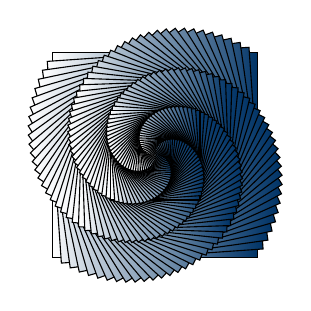
\begin{tikzpicture}
		%\draw[thick, gray] (-1.3,-1.3) rectangle (1.3,1.3);
		%\draw[thick, gray] (-1.6,-1.6) rectangle (1.6,1.6);
		%\fill[black] (2,2) circle (0.5mm);
		
		% Cuadrados más pequeños rotados y escalados
		\foreach \i in {0,1,...,80} {
			\pgfmathsetmacro{\scale}{1- 0.0125*\i}
			\pgfmathsetmacro{\angle}{4*\i}
			\draw[ left color=white, right color=uasdblue, rotate around={\angle:(0,0)}, scale=\scale] (-1.3,-1.3) rectangle (1.3,1.3);
		}
	\end{tikzpicture}
	
	\end{document}